\scanpage{5}

\diagram{\begin{tikzcd}[ampersand replacement=\&,column sep=.7em]
{\mathbb Z[\unsure{\mathbb F|F}_{\unsure{n-2|n\,2|n-1}}]}
\& {\begin{tikzpicture}[baseline=-.15em,x=.45em,y=.45em,line width=.45pt]
\draw (.7,.7)..controls(-.1,.45)and(-.15,-.1)..(.55,-.5);
\draw (.45,.05)--(1.65,.05);
\end{tikzpicture}}
\& {\mathbb Z[\mathbb F_{n-1}]}
\& {\mathbb Z[F_n]}\arrow[l,"{t_n-s_n}"']
\& {\mathbb Z[\mathbb F_{n+1}]}\arrow[l]
\& {\begin{tikzpicture}[baseline=-.1em,x=.25em,y=.25em,line width=.9pt]
\draw (0,0)--(.9,0)--(1.2,-.25);\draw (.15,-.2)--(.1,.35);\draw (.8,-.35)--(.8,.5);
\end{tikzpicture}}
\end{tikzcd}}
% The first connector has an open curved head separated from its shaft.
% The small terminal mark is traced without assigning it punctuation or an operator.

\figure{\begin{tikzpicture}[x=1em,y=1em,line width=.45pt]
\draw (0,.35)..controls(.04,.08)and(.2,-.05)..(.3,-.12);
\draw (.35,-.16)--(.4,-.18);\draw (.48,-.21)--(.6,-.23);
\draw (1.1,.06)--(1.2,.13);\draw (1.28,.2)--(1.48,.32);
\end{tikzpicture}}
% Detached curved traces below the chain; status as intentional lettering is not established.

\[
\begin{aligned}
D_n&\longrightarrow X &\quad&\deleted{D_n}{}^{\boldsymbol\cdot}\\
\bigl\{x&\in F_n && =
\end{aligned}
\]

\[
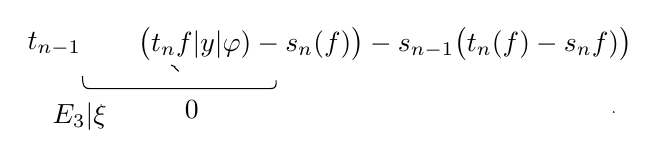
\begin{tikzpicture}[baseline=0pt,x=1em,y=1em,line width=.4pt]
\node[anchor=west,inner sep=0pt] at (0,0) {$t_{n-1}$};
\node[anchor=west,inner sep=0pt] at (4,0) {$\bigl(t_n\unsure{f|y|\varphi})-s_n(f)\bigr)-s_{n-1}\bigl(t_n(f)-s_n f)\bigr)$};
\draw (2,-1.15)..controls(2,-1.55)and(2.1,-1.6)..(2.25,-1.6)--(8.8,-1.6)
 ..controls(9,-1.6)and(9,-1.5)..(9,-1.3);
\node at (1.9,-2.6) {$\unsure{E_3|\xi}$};
\node at (5.95,-2.35) {$0$};
\draw (5.2,-.75)--(5.36,-.82);\draw (5.32,-.83)--(5.48,-.98);
\fill (21.2,-2.45) circle (.035);
\end{tikzpicture}
\]
% Missing inner opening parentheses are retained. The low bracket is traced in its
% physical span; it does not enclose the entire first difference as an underbrace.

\[
\begin{array}{cc}
\underset{\smile}{F}_0 & F_1\\[.6em]
F'_0 & \mathbb F'_1\\
\unsure{\prime|1}&
\end{array}
\]
\diagram{\begin{tikzcd}[ampersand replacement=\&,column sep=1.7em,row sep=1.3ex]
\&\& \unsure{s|f}\&t\arrow[l]\\
{\substack{\exists\,\deleted{\unsure{u|w}}s,u'\\s'}} \&
 f(s)\arrow[l] \& f_0(s) \& f_0(t)\arrow[l]
\end{tikzcd}}

\begin{flushright}
\begin{minipage}{.74\linewidth}
\(\bigl(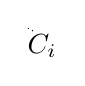
\begin{tikzpicture}[baseline=-.55ex,x=1em,y=1em]
\node[inner sep=0pt] at (0,0) {$C_i$};
\fill (-.5,.65) circle (.025);\fill (-.35,.57) circle (.025);
\end{tikzpicture}\bigr)\quad\forall w'\in\mathbb F'_i,\)
\deleted{si on \unsure{retient|retire}} \(\deleted{s}\exists w\in F_i\) tel que
\(f(w)\sim w'\). De plus si \(i\geq1\), On peut
\par\noindent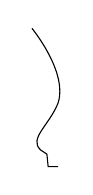
\begin{tikzpicture}[baseline=-2.3em,x=.45em,y=.5em,line width=.4pt]
\draw (0,5)..controls(1.7,3)and(2.6,1)..(2.1,-.4)
 ..controls(1.4,-2)and(-.3,-3)..(.7,-3.8)--(1.2,-4.1)--(1.3,-5)--(2.1,-5);
\end{tikzpicture}\begin{minipage}{.89\linewidth}
se donner d'avance \(u_i=s_i(w)\), \inserted{\(v_i=\)}\(t_i(w)\),
\inserted{de \(F_{i-1}\),} soumis aux seules conditions \deleted{de} que
\(f(u_{\unsure{\cdot|i|1}})=u'_{\unsure{i|1}}\), \inserted{\unsure{rp|resp}}
\(g(v_i)=v'_i\)
et, \deleted{de} plus, si \(i-1\geq1\) i.e \(i\geq2\), \deleted{que}
\(s(u)=s(v),\ t(u)\unsure{\equiv|=}t(v)\)
\end{minipage}

(NB on n'exige pas que \(g(u)=u'\))
\end{minipage}
\end{flushright}
% The two points at the upper left of C are literal marks, not an asserted accent.
% The later two boundary subscripts share the i/1 doubt first marked above.

\[
\begin{aligned}
\unsure{\Xi|E}_0\quad\text{\textcircled{\(\unsure{\mathrm a)|\mathrm b)}\)}}\quad&
\forall s'\in F'_0,\quad \exists s\in\mathbb F_0,\ u\in\mathbb F'_1,\quad
f_0(s)\xrightarrow{u}s'\\[-.1em]
&\hspace{4em}\deleted{\pi_0(f)\ \text{surj}}\quad
-\pi_0(f)\ \text{\uuline{surj}}\\
\mathrm b)\quad&
\forall s,t\in F_0,\quad
\underset{\substack{\rotatebox{90}{\(\in\)}\\F'_1}}{u'}:f_0(s)\longrightarrow f_0(t),\\
&\exists u\in\mathbb F_1,\quad u:s\mathbin{-}t\qquad\pi_0(f)\ \text{inj.}
\end{aligned}
\]

\[
\begin{aligned}
\Xi_1\quad\text{\textcircled{\(\mathrm b')\)}}\quad&
\forall s,t\in F_0,\quad
\underset{\substack{\rotatebox{90}{\(\in\)}\\F'_1}}{u'}:
 f_0(s)\mathbin{-} f_0(t),\\
&\exists u\in F_1,\quad u:s\mathbin{-}t,\quad
 f(u)\mathrel{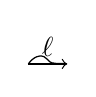
\begin{tikzpicture}[baseline=-.4ex,x=.35em,y=.35em,line width=.45pt]
\draw[->] (0,0)--(4,0);
\draw (0,0)..controls(.7,1.0)and(1.6,1.0)..(2,.45)
 ..controls(2.5,-.25)and(3.4,.2)..(4,0);
\node at (2,1.8) {$\ell$};
\end{tikzpicture}}u'\\
&\deleted{\unsure{\exists\,w|w}\in F_2}\\
&\pi_0(f)\ \text{inj. et }\text{\uuline{\(\pi_1(f)\) surj}}
\end{aligned}
\]
% The first two level glyphs have three separated bars; the E/Xi doubt is marked
% at its first occurrence. The last level glyph below has a visible upright.

\[
\begin{aligned}
\mathrm c)\quad&
\deleted{\forall s,t\in\mathbb F_0,}\ u,v\in\unsure{F|\mathbb F}_1\quad
\begin{gathered}s_i(u)=s_1(v),\\[-.2em] t_1(u)=t_1(v)\end{gathered},\\
&\text{et }\underset{\substack{\rotatebox{90}{\(\in\)}\\F'_2}}{w'}:
 f(u)\longrightarrow f(v),\quad
 \exists\underset{\substack{\rotatebox{90}{\(\in\)}\\F_2}}{w}:
 \deleted{\unsure{f|f_1}}u\mathbin{-}v\\
&\pi_{\unsure{f|1}}(f)\ \text{inj.}
\end{aligned}
\]
\diagram{\begin{tikzcd}[ampersand replacement=\&,column sep=2.4em,row sep=.8em,cells={nodes={inner sep=0pt}}]
{}\arrow[r,bend left=45,"u"]\&{}\\
{}\arrow[r,bend right=45,"v"']\&{}
\end{tikzcd}}

\[
\begin{aligned}
E_2\quad\text{\textcircled{\(\mathrm c'\)}}\quad&
\forall(u,v)\in\mathbb F_1,\quad
\begin{gathered}s_1(u)=s_1(v)\\[-.2em] t_1(u)=t_1(v)\end{gathered}
\quad\text{et }\underset{\substack{\rotatebox{90}{\(\in\)}\\F'_2}}{w'}:
 f(u)\mathbin{-}f(v),\\
&\exists\underset{\substack{\rotatebox{90}{\(\in\)}\\F_2}}{w}:u\longrightarrow v\
 \deleted{et}\ \text{tel que}\\
&w'\sim f(w)
\end{aligned}
\]
\figure{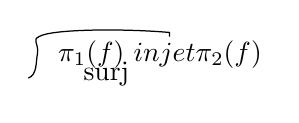
\begin{tikzpicture}[x=.6em,y=.6em,line width=.45pt]
\node[anchor=west] at (1.2,1.1) {$\pi_1(f)\ \text{inj et }\pi_2(f)$};
\node at (4.7,-.05) {surj};
\draw (0,-.3)..controls(.55,-.1)and(.45,.7)..(.55,1.15)
 ..controls(.65,1.8)and(.2,2)..(.65,2.2)
 ..controls(1.35,2.65)and(5.6,2.7)..(8.5,2.45)--(8.5,2.2);
\end{tikzpicture}}
\figure{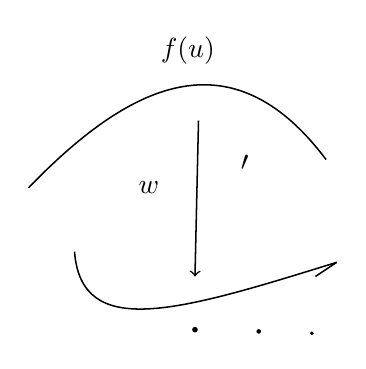
\begin{tikzpicture}[x=.045cm,y=.045cm,line width=.55pt]
\node[anchor=south] at (45,32) {$f(u)$};
\draw (0,0)..controls(28,29)and(57,44)..(84,8);
\draw (13,-18)..controls(15,-43)and(42,-35)..(87,-21);
\draw (87,-21)--(81,-25); % small inward return at the lower right tip
\node at (34,0) {$w$};\node at (61,7) {$\prime$};
\draw[->] (48,19)--(47,-25);
\fill (47,-40) circle (.8);\fill (65,-40.5) circle (.65);\fill (80,-41) circle (.55);
\end{tikzpicture}}
% The lower sketch has separated curve endpoints, w and prime on opposite sides
% of the down stroke, and three detached points beneath the lower curve.
% archive sheet number: 4
% Pale type-like background traces were inspected, including a rotated crop.
% No complete additional typed word is securely recoverable from this face.
